\section{\xxx Background}\label{sec:background}

This section introduces the background of two key techniques in \xxx, the 
\paxos consensus protocol (\S\ref{sec:paxos}) and RDMA features 
(\S\ref{sec:rdma}).

\subsection{\paxos}\label{sec:paxos}
% \paxos background. Keys:
% Leader, backup.
% Persistent storage. 
% Network round trips in normal case. Latency.
An SMR system runs the same program and its data on a set of machines 
(replicas), and it uses a distributed consensus protocol (typically, \paxos) 
to coordinates inputs across replicas. For efficiency, in normal case, \paxos 
often let one replica work as the leader which invoke consensus requests, and 
the other replicas work as backups to agree on or reject these requests. If 
the leader fails, \paxos elects a new leader.

When a new input comes, \paxos starts a new consensus round, which invokes a 
consensus request on this input to the other replicas. \paxos guarantees that 
all replicas consistently agree to process this input as long as a majority of 
replicas' agreement. This quorum based consensus makes \paxos tolerate various 
faults such as machine failures and network crashes. Before a replica agrees on 
a input, \paxos logs this input in the replica's persistent storage for 
durability. As rounds move on, \paxos consistently enforce the same sequence of 
inputs among replicas. If a program runs as a deterministic state machine (\ie, 
given the same input, the program always produces the same output), \paxos 
guarantees that programs on active replicas never diverge.

% Normal case, round trip.
Netork latency of consensus messages is one key challenge to make SMR support 
general server programs which demand high perforrmance, espeically in-memory 
storage servers. Because each input input is processed by a server program, 
existing consensus protocols involve consensus messages on TCP or UDP, which go 
through software network layers and the OS kernel, causing hundreds of \us 
latency in LAN. For instance, even in an efficient \paxos protocol, each input 
in normal case takes two consensus messages between every two replicas (one a 
request from leader to backup and the other a reply from backup to leader).


\subsection{RDMA}\label{sec:rdma}
% RDMA background.
% Cheap, pervasive.
% One-sided write operations. Faster than IPoIB.
RDMA recently has become commonplace in Datacenter networking due to its high 
performance and its decreashing price. For instance, a machine with 40Gbps RDMA 
NIC and 24-cores costs 3.8K US \$, and a RDMA switch with 40Gbps costs about 
16K US \$. RDMA provides three types of communication primitives, including 
IPoIB, message verbs, and one-sided read/write operations, from slow to fast. To 
perform RDMA operations, the process and the remote process establishes a 
communication end point called Queue Pairs (QP). The remote memory access is 
fully operated by hardware without involing software network layers, OS kernel, 
or CPU of the remote machine. QP are lossless in normal case, but packet losses 
may happen during machine or software (\eg, the server program) restarts.

One-side RDMA operations can totally write from one machine's memory to a 
remote machine's memory directly. However, for one-sided operations, the remote 
machine's memory is not aware of the write either, so a careful protocol design 
is necessary when one-sided operations are used.


\section{\xxx Overview}\label{sec:overview}

This section presents an overview of \xxx's architecture with its deployment 
model and key components (\S\ref{sec:arch}), and it gives an example to show 
how it works (\S\ref{sec:example}).

\subsection{Architecture}\label{sec:arch}

\begin{figure*}[!htb]
\centering
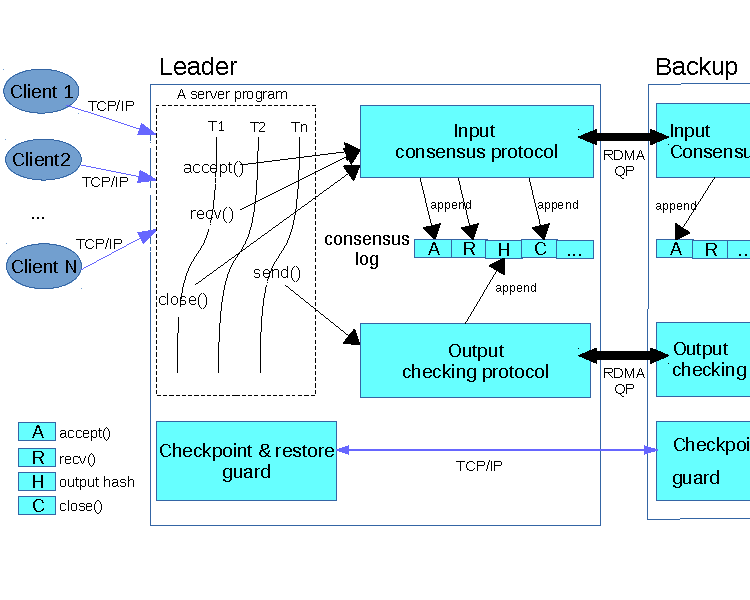
\includegraphics[width=0.5\textwidth]{figures/arch}
\vspace{-.10in}
\caption{{\em The \xxx Architecture.} \rm {\xxx components are shaded (and in
  green).}} \label{fig:arch}
\vspace{-.05in}
\end{figure*}

% TBD. Input coordinator and output checker. Components.

% System model. Replicas. RDMA. LAN. Clients.

% Input coordination protocol.
Figure~\ref{fig:arch} shows \xxx's architecture.

% Output checking protcol.

% The guard component. Checkpoint and restore.


\subsection{Example}\label{sec:example}

% TBD. A simple server with recv(), accept(), and send(). Must have a 
% concurrency bug in this toy program? Race on global var or heap?